%
% idee.tex -- Polynom Idee
%
\section{Idee
\label{reedsolomon:section:idee}}
\rhead{Problemstellung}
Um beim Datenübertragen Fehler zu erkennen, könnte man die Daten jeweils doppelt senden,
    also immer zwei gleich Werte miteinander und so jeweilige einen Fehler zu erkennen.
Wenn jedoch mehr als nur ein Fehler erkennt werden soll und sogar noch das orginal rekonstruiert werden soll,
dann werden die Daten drei oder vierfach versendet.
Doch nur schon um Fehler zu erkennen werden überproportional viele Daten doppelt und dreifach gesendet.
Das Problem liegt darin Informationen, Zahlen, 
    zu Übertragen und Fehler zu erkennen.
Speziell beim Reed-Solomon-Code kann man nicht nur Fehler erkennen, 
    man kann sogar einige Fehler korrigieren.
Der Unterschied des Fehler erkennen und korrigiren, ist das beim Erkennen nur die Frage beantwortet wird: Ist die Übertragung fehlerhaft oder nicht?
Beim Korrigieren werden Fehler erkannt und dann zusätzlich noch den original Wert rekonstruieren.
Der Reed-Solomon-Code macht dies auf eine andere, clevere Weise.
Anwendungen finden sind im Abschnitt \externaldocument{papers/reedsolomon/anwendungen}
\ref{reedsolomon:section:anwendung} beschrieben.

\subsection{Polynom-Ansatz
\label{reedsolomon:section:polynomansatz}}
\rhead{Polynom-Ansatz}
Eine Idee ist, aus den Daten ein Polynom zu bilden. 
In deieser Art arbeitet der Reed-Solomon-Code.
Von dieser Polynomfunktion wird dann eine Anzahl Werte übertragen.
\begin{beispiel} Nehmen wir zum Beispiel die Zahlen \textcolor{blue}{2}, \textcolor{blue}{1}, \textcolor{blue}{5},
    welche uns dann das Polynom 
\begin{equation}
p(x)
=
\textcolor{blue}{2}x^2 + \textcolor{blue}{1}x + \textcolor{blue}{5}
\label{reedsolomon:equation1}
\end{equation}
ergibt.
\par 
Ein Polynome zweiten Grades ist durch drei Punkte eindeutig bestimmbar. 
Bei einer fehlerlosen Übertragung, können wir mit 3 übertragene Werte,
    das Polynom durch Polynominterpolation volständig rekonstruieren.
Weder erkläre noch erläutere ich die Polynominterpolation, 
    sie kann nachgeschaut werden oder als Funktion angewendet werden.
Die koeffizente, des rekonstruierten Polynoms, sind dann unsere gesendten Zahlen \textcolor{blue}{2}, \textcolor{blue}{1}, \textcolor{blue}{5}.
Wie können wir nun Fehler erkennen oder sogar korrigieren?
Versuchen wir doch mehr Werte zu Übertragen, wir nehmen im Beispiel 7 Werte.
Übertragen werden nun die \textcolor{darkgreen}{grünen Werte} 
    dieses 7 Werte \textcolor{blue}{blauen Polynomes} an den Stellen 1, 2, 3\dots 7 dieses Polynomes.
Grafisch sieht man dies dann in Abbildung \ref{fig:polynom}, 
    mit den Punkten, $p(1),p(2),...,p(7) = (\textcolor{darkgreen}{8}, 
    \textcolor{darkgreen}{15}, \textcolor{darkgreen}{26},
    \textcolor{darkgreen}{41}, \textcolor{darkgreen}{60}, 
    \textcolor{darkgreen}{83}, \textcolor{darkgreen}{110})$
Nun wird durch drei der 7 Punkte das Polynom eindeutig bestimmbar und 
    alle anderen müssen auf diesem Polynom liegen.
Dabei gingen wir von keinem Fehler aus,
    hat es Fehler in der Übertragunge gegeben.
Wir erhöhen nun die Fehleranzahl Schritt für Schritt:
\begin{enumerate}
    \item \textit{Fehler} können konkurenzierende Polynome, zusammen mit zwei originalen Punkten fehlleiten.
        Dabei kann aber maximal 3 Punkte auf diesem Konkurrenzpolynom sein, 
        ansonsten ist der Fehler ein Orginalpunkt und somit kein Fehler.
        Da 6 übereinstimende grössser als 3 ist haben wir unser original Polynom gefunden.
        \par Orginal mit 6 Punkte > 3 Punkte Konkurrenzpolynom, Original Polynom gefunden
        Damit ist klar das unser Polynom mit 6 Punkten richtig ist und unser Fehler kann rekonstruiert werden.
    \item \textit{Fehler} kann ein Fehler mit zwei originalen Punkten ein fehlleitendes Konkurrenzpolynom bilden.
        Da der zweite Fehler frei wählbar ist kann dieser auch auf dem Konkurrenzpolynom liegen, wie in der Abbilbung \ref{fig:polynom}.
        Nun haben wir, wie in unserer Grafik \ref{fig:polynom}, ein Polynom mit 5 übereinstimmenden und eines mit 4 Punkten.
        Da 5 noch grösser als 4 ist, können wir sagen welches das original Polynom ist.
        \par Orginal mit 5 Punkte > 4 Punkte Konkurrenzpolynom, Original Polynom gefunden
    \item \textit{Fehler} kann genau wie bei 2 Fehler, ein Fehler ein fehlleitendes Polynom mit 2 original Punkten bestimmen werden.
        Auch hier sind die anderen Fehler frei wählbar und liegen auf dem Konkurrenzpolynom.
        Nun ist es so das 5 Punkte auf diesem konkurenzierenden Polynom und 4 Punkte auf dem Originalen.
        Das Original Polynom kann nicht mehr gefunden werden.
        \par Orginal mit 5 Punkte > 4 Punkte Konkurrenzpolynom, Original Polynom nicht gefunden
    \item \textit{Fehler} Es kann noch erkennt weden das Fehler statt gefunden haben, da 3 orginale Punkte das ursprüngliche Polynom ergeben.
        Somit haben wir mindestens 2 verschieden Polynome, dass bedeutet Fehler sind entstanden.
    \item \textit{Fehler} Mit den 2 originalen Punkte kann das Originale Polynom nicht mehr erkannt werden und 
        somit auch keine Aussgae gemacht werden ob Fehler statt gefunden haben oder nicht.
\end{enumerate}

\begin{figure}%[!ht]
	\centering
	%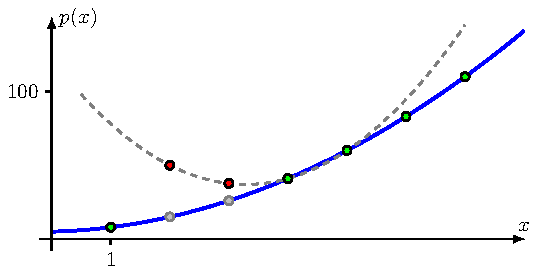
\includegraphics[width=\textwidth]{papers/reedsolomon/figures/polynom2}
    % polynomraw

\newcommand{\teiler}{40}


%//////////////////////////////////////

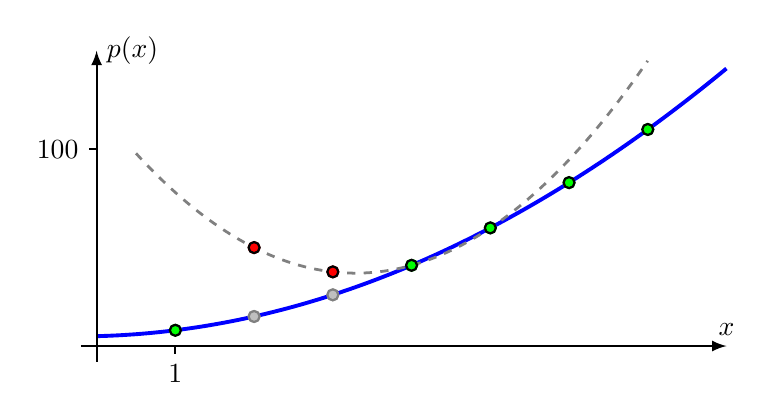
\begin{tikzpicture}[>=latex,thick,]
	\draw[color=blue, line width=1.4pt] 
	plot[domain=0:8, samples=100]
	({\x},{(2*\x^2+1*\x+5)/\teiler});

	\draw[->] (-0.2,0) -- (8,0) coordinate[label={$x$}];
	\draw[->] (0,-0.2) -- (0,150/\teiler) coordinate[label={right:$p(x)$}];
	
	\def\punkt#1{
		\fill[color=green] #1 circle[radius=0.08];
		\draw #1 circle[radius=0.07];
	}

	\def\hellpunkt#1{
		\fill[color=lightgray] #1 circle[radius=0.08];
		\draw[gray] #1 circle[ radius=0.07];
	}
	
	\draw[color=gray,line width=1pt,dashed] 
	plot[domain=0.5:7, samples=100]
	({\x},{(7.832*\x^2-51.5*\x+121.668)/\teiler});


	\punkt{(1,8/\teiler)}
	\hellpunkt{(2,15/\teiler)}
	\hellpunkt{(3,26/\teiler)}
	\punkt{(4,41/\teiler)}
	\punkt{(5,60/\teiler)}
	\punkt{(6,83/\teiler)}
	\punkt{(7,110/\teiler)}
	

	
	\def\erpunkt#1{
		\fill[color=red] #1 circle[radius=0.08];
		\draw #1 circle[radius=0.07];
	}
	\erpunkt{(2,50/\teiler)}
	\erpunkt{(3,37.66/\teiler)}

	\draw(0,100/\teiler) -- (-0.1,100/\teiler) coordinate[label={left:$100$}];
	\draw(1,0) -- (1,-0.1) coordinate[label={below:$1$}];		
\end{tikzpicture}
	\caption{Polynom $p(x)$ von der Gleichung\eqref{reedsolomon:equation1}}
	\label{fig:polynom}
\end{figure}

\section{Fehlerkorekturstellen bestimmen
\label{reedsolomon:section:Fehlerkorrekturstellen}}
Um zu bestimmen wieviel zusätzliche \textcolor{darkgreen}{Übertragungspunkte} notwendig sind, um die Fehler zu korrigieren,
    muss man zuerst wissen, wieviel \textcolor{blue}{Daten} gesendet und wieviel \textcolor{red}{Fehler} erkennt werden sollen. 
Die Anzahl \textcolor{blue}{Daten} (ab hier verwenden wir das Wort Nutzlast), die als Polynomkoeffizente $k$ übergeben werden, 
    brauchen die gleiche Anzahl an Polynomkoeffizententräger, beginnend bei Grad 0 somit ergibt sich der Polynomgrad mit $k-1$.
Für die Anzahl der Fehler $t$, welche korrigiert werden können, gehen wir zum Beispiel.
\begin{beispiel} von den Polynom \ref{reedsolomon:equation1} in, welchem wir  \textcolor{darkgreen}{7 Übertragungspunkte} senden.
Durch 3 Punkte wird das Polyom eindeutig bestimmt, nun haben wir mehrere Konkurrenzpolynome, doch mit maximal 2 Fehler liegen auf einem Konkurrenzpolynom,
    maximal 4 Punkte und auf unserem orginal 5 Punkte. Ansonsten hatt es mehr Fehler oder unser Konkurrenzpolynom ist das gleiche wie das Original. 
Somit können wir nun bestimmen, dass von den \textcolor{darkgreen}{7 Übertragungspunkten$u$} bis zu 2 Fehler korrigiert werden können und 4 Übertragungspunkte zusätzlich gesendet werden müssen.
\end{beispiel}
Man könnte auch dies in der Tabelle \ref{tab:fehlerkorrekturstellen} erkennen, doch mit dieser Gleichung
\begin{equation}
    \frac{\textcolor{darkgreen}{u}-\textcolor{blue}{k}}{\textcolor{red}{t}}
    =2
    \label{reedsolomon:equation2}
\end{equation}
    zeigt sich, dass es $k+2t$ Übertragungspunkte braucht.

\begin{table}
    \centering
    \begin{tabular}{ c c | c} 
        \hline
        Nutzlas & Fehler & Übertragen \\
        \hline 
        3 & 2 & 7 Werte eines Polynoms vom Grad 2 \\ 
        4 & 2 & 8 Werte eines Polynoms vom Grad 3 \\
        3 & 3 & 9 Werte eines Polynoms vom Grad 2 \\ 
        \hline
        $k$ & $t$ & $k+2t$ Werte eines Polynoms vom Grad $k-1$ \\ 
        \hline
    \end{tabular}
    \caption{ Fehlerkorrekturstellen Bestimmung.}
    \label{tab:fehlerkorrekturstellen}
\end{table}

Ein Nebeneffekt ist, dass dadurch auch $2t$ Fehler erkannt werden können, nicht aber korrigiert.
Um aus den übertragenen Zahlen wieder die Nutzlastzahlen zu bekommen könnte man eine Polynominterpolation anwenden,
doch die Punkte mit Polynominterpolation zu einem Polynom zu rekonstruieren ist schwierig und fehleranfällig.

